\chapter{Hero Run Data Analysis} 
\label{chapter5}

Talk about the fully scaled version of Early Earth: the HiPerGator \textit{hero run}

\section{Molfind}

\subsection{GraphMatcher}

\subsection{Parallelization}


\section{Restarts -- Quench analysis}


\section{Exploring new molecular configurations}
\hypertarget{configurational_sampling}{Sample hyperlink target}

\section{Interpretation of results}



this is the \angstrom in a sentence

\begin{figure}[!ht]
    \centering
    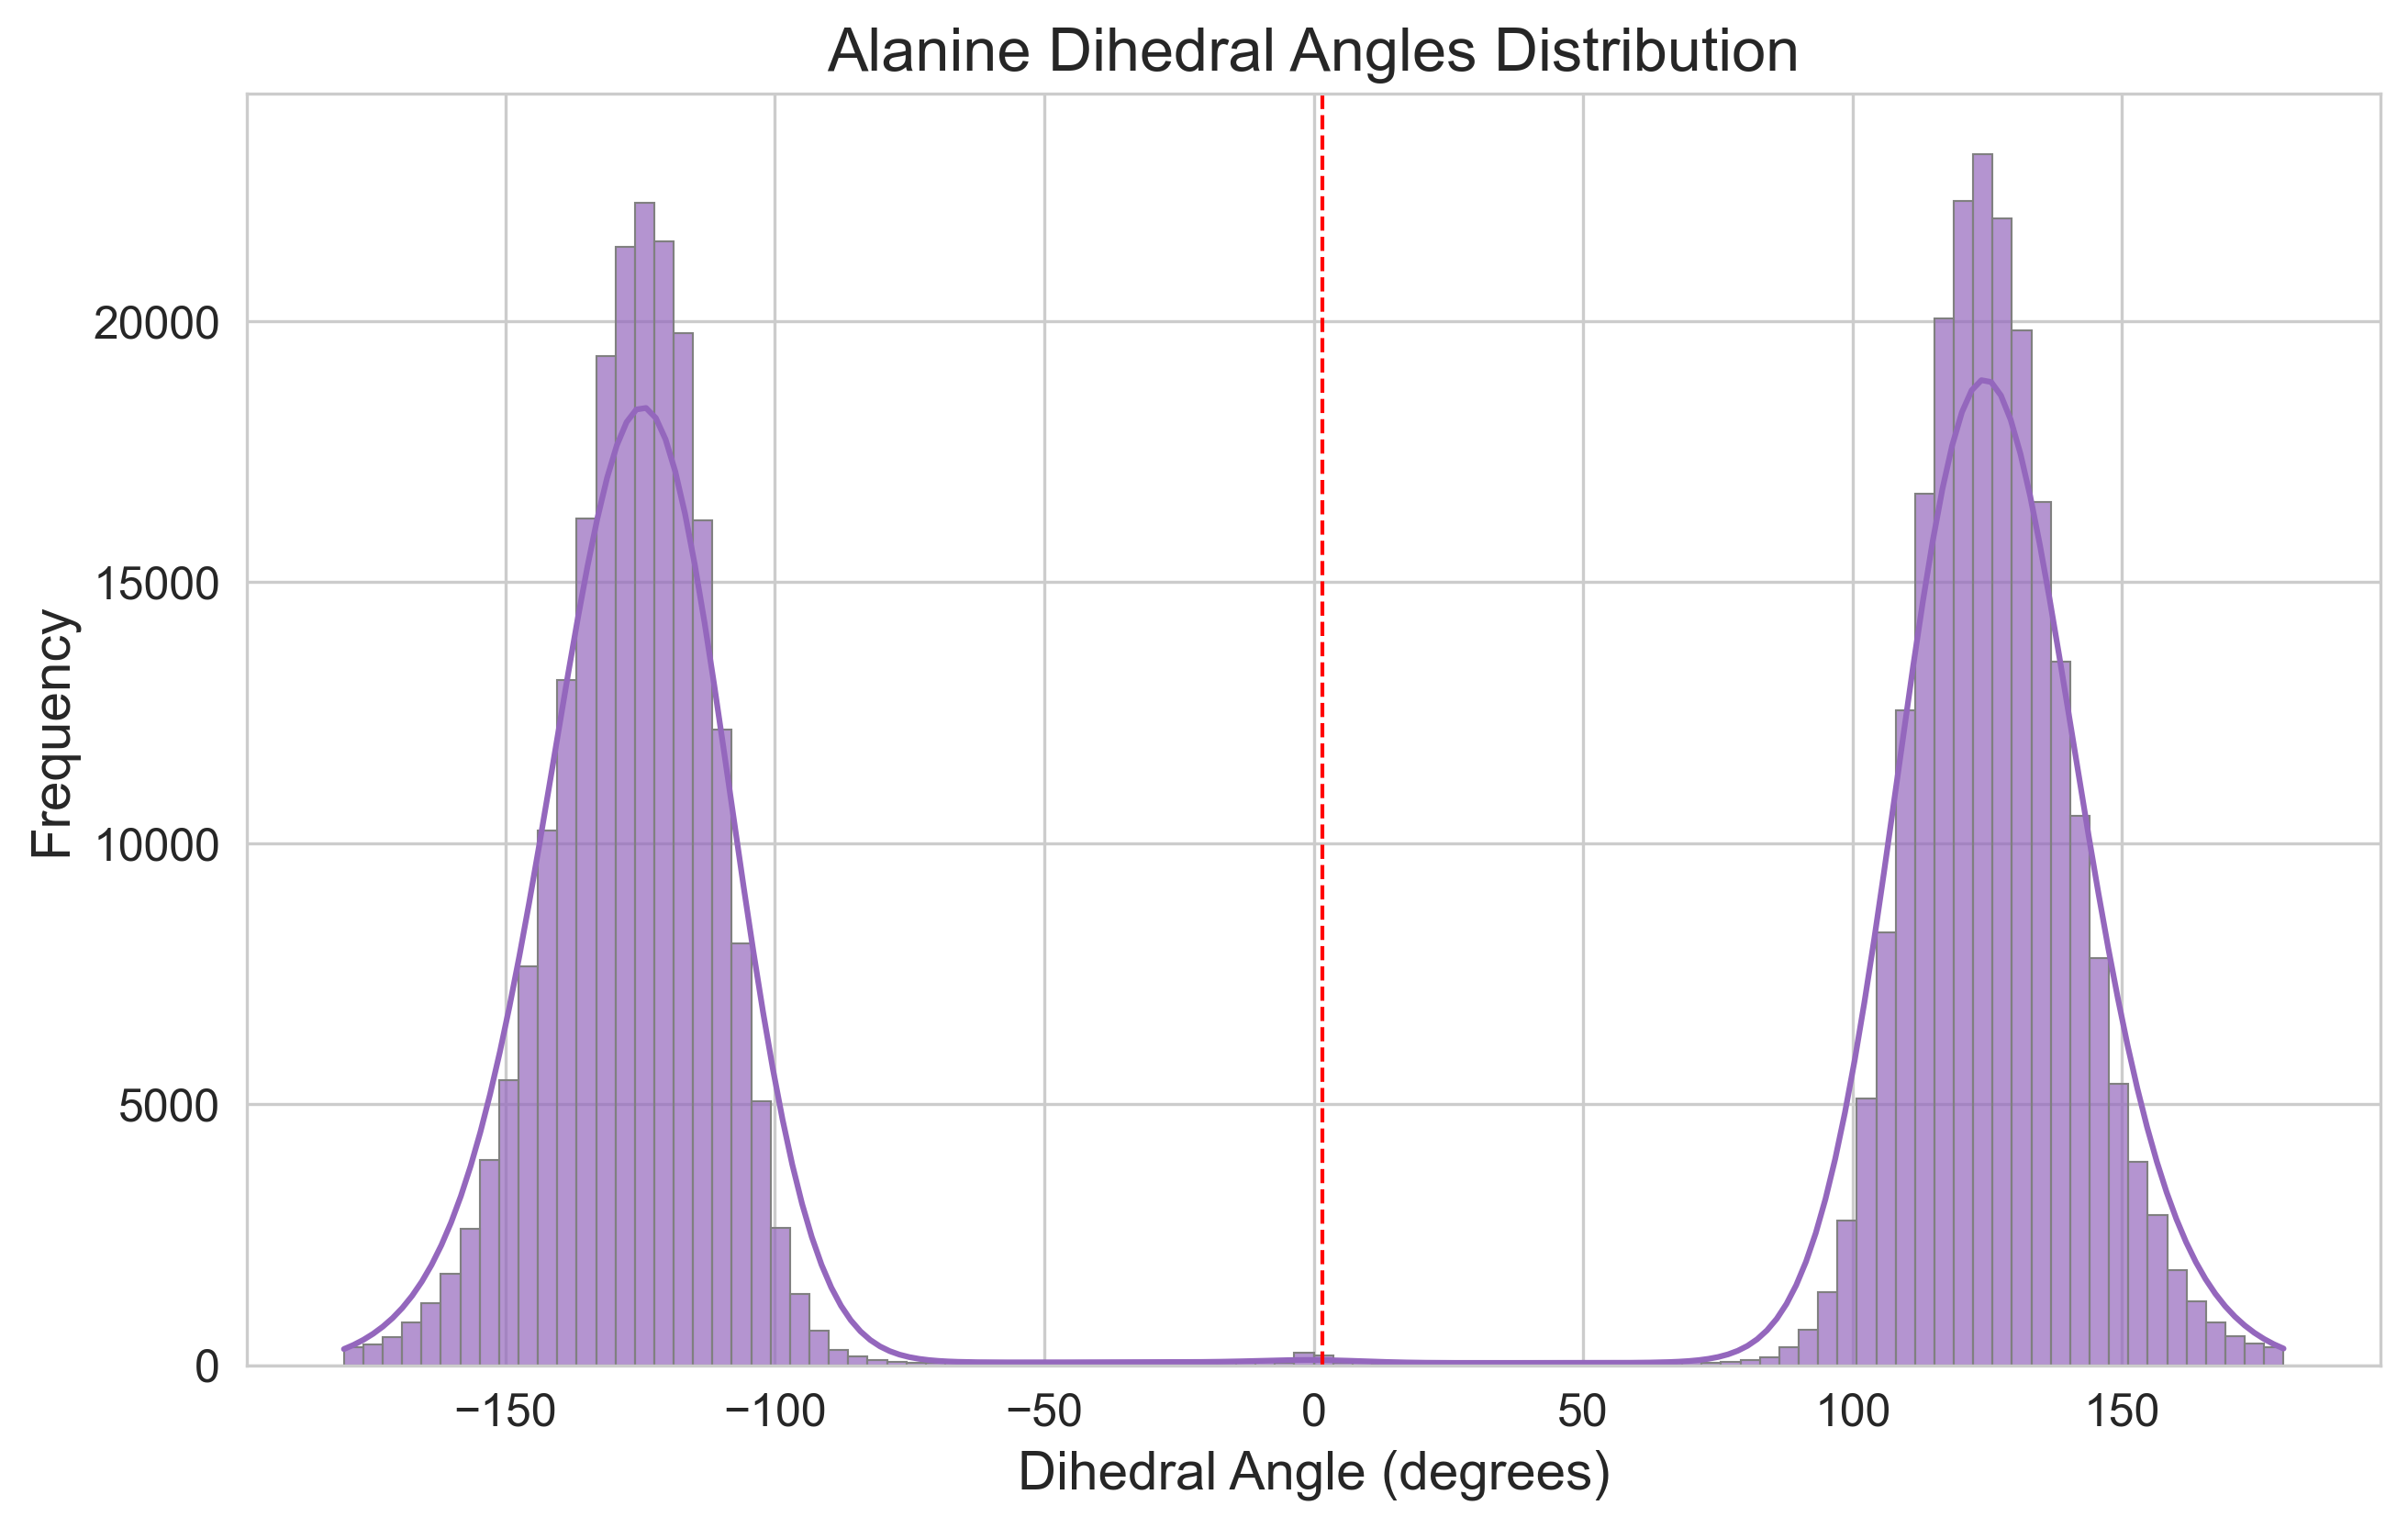
\includegraphics[width=1\linewidth]{Images/useful figures/alanine_dihedral/dihedral_angles_distribution.png}
    \caption{Distribution of dihedral angles in alanine molecules synthesized in the early earth simulation run. All molecules fall within the expected range of dihedral angles, centered at $\pm$125$^\circ$.}
    \label{ala_dihedral}
\end{figure}{}

